\documentclass{article} % Default font size and left-justified equations
% \documentclass{book}

\usepackage[
  margin=0.7in,
  % includefoot,
  % footskip=30pt,
]{geometry}

\usepackage{natbib}
\usepackage{enumitem}
\usepackage{amsmath,amsfonts}
\usepackage{graphicx}
\usepackage{framed}
\usepackage{subcaption}
\usepackage[T1]{fontenc}%
\usepackage[utf8]{inputenc}%
\usepackage{mathrsfs}%
\usepackage{amssymb}%
\usepackage{amsthm}%
\usepackage{graphicx}
\usepackage{hyperref}
\usepackage{environ}
\usepackage{framed}
\usepackage{mdframed} 
\usepackage{wrapfig} 
\usepackage{booktabs}
\usepackage{tabularx} 
\usepackage{array}
\usepackage[font=small]{caption} 
\usepackage{xspace}  
\usepackage[osf,sc]{mathpazo}
\usepackage{pbox}
\usepackage{listings}
\usepackage{tikz}
\usepackage{bm}
\usepackage[strict]{changepage}
\usepackage{mleftright}
\usepackage{appendix}%
\usepackage[all]{xy} 
\setcounter{tocdepth}{3}
\setcounter{secnumdepth}{3}
\usepackage[ruled,vlined]{algorithm2e}
\usepackage{framed}
\usepackage{wrapfig}
\usepackage{pythonhighlight}
\usepackage{tikz}
\usetikzlibrary{arrows}
\usetikzlibrary{arrows.meta}
\usetikzlibrary{shapes.geometric}
\usetikzlibrary{positioning, arrows, automata, calc}
\usepackage{transparent}
\usepackage[many]{tcolorbox}
\usepackage{tikz}
\usetikzlibrary{shapes.geometric}
\usetikzlibrary{positioning, arrows, automata, calc}

\newtcolorbox[]{your_solution}[1][]{
    % breakable,
    enhanced,
    nobeforeafter,
    colback=white,
    title=Your Answer,
    sidebyside align=top,
    box align=top,
    #1
}
\newcommand{\mybox}[1]{
\noindent
\fbox{\parbox{0.955\textwidth}{%
\noindent\texttt{#1}
}
}
}

\newcommand{\filler}{ . . . . . }
\newcommand{\choice}{\hspace{0.5cm}$\square$}
\newcommand{\identity}{\mathbf{I}} 
\newcommand{\paran}[1]{\left( #1 \right)}

%% PLEASE USE THESE MACROS WHEN WRITING THE SOLUTIONS 
\newcommand{\solution}[1]{\textcolor{blue}{Answer: \em #1}
} % show
%\newcommand{\solution}[2]{#2} % hide

\newcommand{\extracredit}{{\color{purple}\textbf{Extra Credit:}}}

\newcommand{\additionalNotes}{
\noindent\textbf{How to hand in your written work:} via MyClasses.  \\ 


\noindent\textbf{Collaboration:} Make certain that you understand the course collaboration policy, described on the course website. 
You may discuss the homework to understand the problems and the mathematics behind the various learning algorithms, but you are \textcolor{red}{\textbf{not allowed to share problem solutions with any other students. You must write the solutions \textbf{individually}}}. \\ 

\noindent\textbf{Typesetting:} 
We strongly recommend typesetting your homework, especially if you have sloppy handwriting. 
% We recommend using LaTeX, but you are welcome to use whatever program and/or markup language you like. 
We will provide a LaTeX template for homework solutions. Type your answers into the corresponding solution field under each question.
}

\title{ \Large COSC490LLMs }
\date{\\ 
\normalsize Name: \_\_\_\_\_\_\_\_\_Kyle Tranfaglia\_\_\_\_\_\_\_\_\_\_\_\_\_\_\_\_\_\_\_\_\_\_\_\_\_\_\_\_\_\_\_    \\ 
Collaborators, if any: \_\_\_\_\_\_Dustin O'Brien (Math discussion)\_\_\_\_\_\_\_\_\_\_\_\_\_\_ \\ 
Sources used for your homework, if any: \_\_\_\_ChatGPT (numpy and pytorch documentation and examples/explainations) \_\_\_\_\_\_\_\_\_\_\_\_\ 
}

\newcommand{\todo}{\textcolor{blue}{\textbf{TODOs}}}



\usepackage{macros}
\usepackage{listings}
\usepackage{xcolor}

\definecolor{codegreen}{rgb}{0,0.6,0}
\definecolor{codegray}{rgb}{0.5,0.5,0.5}
\definecolor{codepurple}{rgb}{0.58,0,0.82}
\definecolor{backcolour}{rgb}{0.95,0.95,0.92}

\lstdefinestyle{mystyle}{
    backgroundcolor=\color{backcolour},   
    commentstyle=\color{codegreen},
    keywordstyle=\color{magenta},
    numberstyle=\tiny\color{codegray},
    stringstyle=\color{codepurple},
    basicstyle=\ttfamily\footnotesize,
    breakatwhitespace=false,         
    breaklines=true,                 
    captionpos=b,                    
    keepspaces=true,                 
    numbers=left,                    
    numbersep=5pt,                  
    showspaces=false,                
    showstringspaces=false,
    showtabs=false,                  
    tabsize=2
}

\lstset{style=mystyle}

\author{
\Large
Homework 1: Background Review + Building a classifier 
}


\begin{document}
% \bibliographyunit[\chapter] % for bibliographies at the end of each chapter

\maketitle

% \emph{Commentary on Homework 1}:
This assignment combines knowledge and skills across several disciplines. 
The purpose of this assignment is to make sure you are prepared for this course. We anticipate that each
of you will have different strengths and weaknesses, so don't be worried if you struggle with \emph{some} aspects
of the assignment. But if you find this assignment to be very difficult overall, that is an early warning sign that you may not be prepared to take this course at this time. \\ 
% Future assignments will be more difficult than this one (and probably around the same length).

To succeed in the course, you will need to know or very quickly get up to speed on:
\begin{itemize}
\item Math to the level of the course prerequisites: linear algebra, multivariate calculus, some probability.
\item Statistics, algorithms, and data structures to the level of the course prerequisites.
\item Python programming, and the ability to translate from math or algorithms to programming and back.
\item Some basic LaTeX skills so that you can typeset equations and submit your assignments.
\end{itemize}

% Questions 1-4 are on review material, that we expect you to know coming into the course. The rest is related to the first few lectures.

% \noindent\fbox{
%     \parbox{\textwidth}{
%         \textbf{Homework goals:} After completing this homework, you should be comfortable with: 
%         \begin{itemize}
%             \item 
%         \end{itemize}
%     }
% }

\vspace{0.5cm}

\additionalNotes


\clearpage



\section{Refreshing the Rows and Columns: Linear Algebra Review}

For these questions, you may find it helpful to review  \href{http://www.cs.ubc.ca/~schmidtm/Documents/2009_Notes_LinearAlgebra.pdf}{these notes on linear algebra}. 



\subsection{Basic Operations}

Use the definitions below,
\[
\alpha = 2,\quad
\x = \left[\begin{array}{c}
0\\
1\\
2\\
\end{array}\right], \quad 
\y = \left[\begin{array}{c}
3\\
4\\
5\\
\end{array}\right],\quad
\textbf{z} = \left[\begin{array}{c}
1\\
2\\
-1\\
\end{array}\right],\quad
A = \left[\begin{array}{ccc}
3 & 2 & 2\\
1 & 3 & 1\\
1 & 1 & 3
\end{array}\right],
\]
and use $x_i$ to denote element $i$ of vector $\x$.
Evaluate the following expressions:
\begin{enumerate}
    \item $\sum_{i=1}^n x_iy_i$ (inner product).
    \solution{$14$}
    
    \item $\sum_{i=1}^n x_iz_i$ (inner product between orthogonal vectors).
    \solution{$0$} 
    
    \item $\alpha(\x+\y)$ (vector addition and scalar multiplication).
    \solution{\left[\begin{array}{c}
6\\
10\\
14\\
\end{array}\right]}

    \item $\norm{\x}$ (Euclidean norm of $x$).
    \solution{$\sqrt{5}$$}
    
    \item $\x^\top$ (vector transpose).
    \solution{\begin{bmatrix}
        0 & 1 & 2
    \end{bmatrix}}

    \item $A\x$ (matrix-vector multiplication).
    \solution{\left[\begin{array}{c}
6\\
5\\
7\\
\end{array}\right]}

    \item $\x^\top A\x$ (quadratic form).
    \solution{$19$}
\end{enumerate}
Note, you do not need to show your work. 

\begin{wraptable}[7]{r}{7.2cm}
 \begin{framed}
 \footnotesize
In the realm where self-supervision crafts,\\ 
You'll need some skills to climb its shafts. \\ \\
Firstly, you'll need your linear algebra potion, \\ 
Ready to solve with matrix motion. \\ 
Eigenvalues, vectors, and spaces we'll trek, \\ \\
Then we venture into probability's domain, \\ 
Where uncertainty and statistics maintain. \\ 
Random variables, distributions so fair,  \\ \\
Then you must program, in PyTorch, no less, \\ 
% Create neural networks, iterate and assess. \\ 
Tensors, data loaders: your new-found friends,\\ 
Backpropagation till the very end.  \\

\hspace{3.5cm}---GPT-4 Jan 8 2024 
\end{framed}
\end{wraptable}
\subsection{Matrix Algebra Rules}

Assume that $\set{\x, \y, \z}$ are $n \times 1$ column vectors and $\{A, B, C\}$ are $n \times n$ real-valued matrices, 
% $0$ is the zero matrix of appropriate size, and 
and $\identity$ is the identity matrix of appropriate size. State whether each of the below is true in general (you do not need to show your work).

\begin{enumerate}
    \item $\x^\top \y = \sum_{i=1}^n x_iy_i$.
    \solution{True}
    
    \item $\x^\top \x = \norm{\x}^2$.
    \solution{True}
    
    \item $\x^\top \x = \x\x^\top$.
    \solution{False}
    
    \item $(\x-\y)^\top(\y-\x) = \norm{\x}^2 - 2\x^\top \y + \norm{\y}^2$.
    \solution{True}
    
    \item $AB=BA$.
    \solution{False}
    
    \item $A(B + C) = AB + AC$.
    \solution{True}
    
    \item $(AB)^\top = A^\top B^\top$.
    \solution{False}
    
    \item $\x^\top A\y = \y^\top A^\top \x$.
    \solution{True}
    
    \item $A^\top A = \identity$ if the columns of $A$ are orthonormal.
    \solution{True}
\end{enumerate}

\clearpage


\subsection{Matrix operations}
Let 
$\textbf{B} = 
\begin{bmatrix}
1 & -1 & 0 \\  
-1 & 2 & -1 \\ 
0 & -1 & 1
\end{bmatrix}$. 
    Is $\textbf{B}$ invertible? If so, find $\textbf{B}^{-1}$. 
    \solution{\[
\begin{bmatrix}
1 & -1 & 0 \\  
-1 & 2 & -1 \\ 
0 & -1 & 1
\end{bmatrix} \rightarrow \begin{bmatrix}
1 & -1 & 0 \\  
0 & 1 & -1 \\ 
0 & -1 & 1
\end{bmatrix}  \rightarrow \begin{bmatrix}
1 & -1 & 0 \\  
0 & 1 & -1 \\ 
0 & 0 & 0
\end{bmatrix}\]
\textbf {Since we reach at state where row 2 of the matrix is all zeros, we can conclude that B is not invertible as identity matrix, I,  cannot be reached with reduction of matrix B.} \\
}

Is $\textbf{B}$ diagonalizable? If so, find its diagonalization. 
 \\ \\ \text{To determine if \(\mathbf{B}\) is diagonalizable, we must find its eigenvalues and eigenvectors. Thus, we calculate:}
\[
\det(\mathbf{B} - \lambda I) = 
\begin{vmatrix}
1-\lambda & -1 & 0 \\
-1 & 2-\lambda & -1 \\
0 & -1 & 1-\lambda
\end{vmatrix}
\]

Using an online matrix computational tool, we get the eigenvalues: \(\lambda_1 = 0\), \(\lambda_2 = 1\), \(\lambda_3 = 3\).

Now, solving for eigenvectors, we find:
\[
\mathbf{v}_1 = \begin{bmatrix} 1 \\ 1 \\ 1 \end{bmatrix}, \quad
\mathbf{v}_2 = \begin{bmatrix} -1 \\ 0 \\ 1 \end{bmatrix}, \quad
\mathbf{v}_3 = \begin{bmatrix} 1 \\ -2 \\ 1 \end{bmatrix}.
\]

Using the eigenvectors to form matrix \(P\) and the eigenvalues to form \(D\):
\[
P = \begin{bmatrix}
1 & -1 & 1 \\
1 & 0 & -2 \\
1 & 1 & 1
\end{bmatrix}, \quad
D = \begin{bmatrix}
0 & 0 & 0 \\
0 & 1 & 0 \\
0 & 0 & 3
\end{bmatrix}.
\]

Next, we compute \(P^{-1}\) as:
\[
P^{-1} = \frac{1}{\det(P)} \cdot \text{adj}(P) = \begin{bmatrix}
1/3 & 1/3 & 1/3 \\
-1/2 & 0 & 1/2 \\
1/6 & -1/3 & 1/6
\end{bmatrix}.
\]
\solution{
Finally, we verify:
\[
P D P^{-1} = \begin{bmatrix}
1 & -1 & 0 \\
-1 & 2 & -1 \\
0 & -1 & 1
\end{bmatrix},
\]
which matches the original matrix \(\mathbf{B}\), confirming its diagonalization.
}

\newpage

\section{Taking Chances: Probability Review}

% For these questions you may find it helpful to review these notes on probability:\\
% \url{http://www.cs.ubc.ca/~schmidtm/Courses/Notes/probability.pdf}\\
% And here are some slides giving visual representations of the ideas as well as some simple examples:\\
% \url{http://www.cs.ubc.ca/~schmidtm/Courses/Notes/probabilitySlides.pdf}

% \subsection{Rules of probability (? pts)}

\subsection{Basic probability}
Answer the following questions. You do not need to show your work.

\begin{enumerate}
    \item You are offered the opportunity to play the following game: your opponent rolls 2 regular 6-sided dice. If the difference between the two rolls is at least 3, you win \$15. Otherwise, you get nothing. What is a fair price for a ticket to play this game once? In other words, what is the expected value of playing the game?
    \solution{\$5}
    
    \item Consider two events $A$ and $B$ such that $\Pr(A, B)=0$ (they are mutually exclusive). If $\Pr(A) = 0.4$ and $\Pr(A \cup B) = 0.95$, what is $\Pr(B)$? Note: $p(A, B)$ means ``probability of $A$ and $B$'' while $p(A \cup B)$ means ``probability of $A$ or $B$''. It may be helpful to draw a Venn diagram.
    \solution{$\Pr(B)$ = 0.55}
    
    \item Instead of assuming that $A$ and $B$ are mutually exclusive ($\Pr(A,B) = 0)$, what is the answer to the previous question if we assume that $A$ and $B$ are independent?
    \solution{$\Pr(B) = \frac{0.55}{0.6} \approx 0.9167$}
\end{enumerate}


\subsection{Expectations and Variance}

Suppose we have two coins. Coin $C_1$ comes up heads with probability $0.3$ and coin $C_2$ comes up heads with probability $0.9$. We repeat this process 3 times:
\begin{itemize}
    \item Choose a coin with equal probability. 
    \item Flip that coin once. 
\end{itemize}

Suppose $X$ is the number of heads after 3 flips.
\begin{enumerate}
    \item What is $\expec{X}$?
    \item What is $\var{X}$?
    \item Based on the number of heads we get, we earn $Y = \frac{1}{2 + X}$ dollars. 
    What is $\expec{Y}$?
\end{enumerate}

\solution{\\ $1. P(H) = P(C_1) \cdot P(H \mid C_1) + P(C_2) \cdot P(H \mid C_2) \rightarrow
P(H) = 0.5 \cdot 0.3 + 0.5 \cdot 0.9 = 0.15 + 0.45 = 0.6 \rightarrow E[X] = 3 \cdot P(H) = 3 \cdot 0.6 = 1.8 \\ \\
2. \text{Var(H)} = P(H) \cdot (1 - P(H)) = 0.6 \cdot (1 - 0.6) = 0.6 \cdot 0.4 = 0.24 \rightarrow \text{Var[X]} = 3 \cdot \text{Var(H)} = 3 \cdot 0.24 = 0.72 \\ \\
3. E[Y] = \sum_{k=0}^3 \frac{1}{2 + k} \cdot P(X = k) \rightarrow
E[Y] = \frac{1}{2} \cdot 0.064 + \frac{1}{3} \cdot 0.288 + \frac{1}{4} \cdot 0.432 + \frac{1}{5} \cdot 0.216 \rightarrow
E[Y] = 0.032 + 0.096 + 0.108 + 0.0432 = 0.2792
$}

\subsection{A Variance Paradox?}

For independent identically distributed (i.i.d.) random variables $X_1, ..., X_n$, each with distribution $F$ and variance $\sigma^2$.
We know that $\var{X_1 + ... + X_n} = n\sigma^2$. 
On the other hand, if $X \sim F$, then $\var{X + X} = \var{2X} = 4 \sigma^2$. Is there a contradiction here? Explain. 

\solution{
There is no contradiction here. Given $\var{X_1 + ... + X_n} = n\sigma^2$ and $X_1, ..., X_n$ are independent with a variance of $\sigma^2$, it follows the property of independent random variables such that $Var(X + Y) = Var(X) + Var(Y)$. However, if $X \sim F$ with a variance of $\sigma^2$ and we say $\var{X + X} = \var{2X} = 4 \sigma^2$, there is no contradiction as there is a perfect correlation (dependence) since X is summed with itself, producing a scalar of 4 to apply to the variance. Thus, since the first case has independent variables and the second case has dependent variables, the behavioral difference leading to a scaling of variance by 4 rather than n is expected and consistent with the properties of the variance. Therefore, there is no contradiction.
}

\newpage

\section{Calculus Review }
 
\subsection{One-variable derivatives}

Answer the following questions. You do not need to show your work.

\begin{enumerate}
    \item Find the derivative of the function $f(x) = 3x^2 -2x + 5$.
    \solution{$f'(x) = 6x - 2$}
    
    \item Find the derivative of the function $f(x) = x(1-x)$.
    \solution{$f'(x) = 1 - 2x$}
    
    \item Let $p(x) = \frac{1}{1+\exp(-x)}$ for $x \in \reals$. Compute the derivative of the function $f(x) = x-\log(p(x))$ and simplify it by using the function $p(x)$.
    \solution{$f'(x) = 1 - \frac{\exp(-x)}{1 + \exp(-x)} = 1 - \exp(-x) \cdot p(x)$}
\end{enumerate}
Note that in this course we will use $\log(x)$ to mean the ``natural'' logarithm of $x$, so that $\log(\exp(1)) = 1$. Also, observe that $p(x) = 1-p(-x)$ for the final part.

\subsection{Multi-variable derivative}

Compute the gradient $\nabla f(\x)$ of each of the following functions. You do not need to show your work.
\begin{enumerate}
    \item $f(\x) = x_1^2 + \exp(x_2)$ where $\x = [x_1, x_2] \in \reals^2$.
    \solution{$ \nabla f(x) =
    \begin{bmatrix}
    2x_1 \\
    e^{x_2}
    \end{bmatrix}
    $}
    \item $f(\x) = \exp(x_1 + x_2x_3)$ where $\x = [x_1, x_2, x_3] \in \reals^3$.
    \solution{$ \nabla f(x) =
    \begin{bmatrix}
    e^{(x_1 + x_2 x_3)} \\
    x_3 e^{(x_1 + x_2 x_3)} \\
    x_2 e^{(x_1 + x_2 x_3)}
    \end{bmatrix}
    $}
    
    \item $f(\x) = \mathbf{a}^\top \x$ where $\x \in \reals^2$ and $\mathbf{a} \in \reals^2$.
    \solution{$ f(x) = a_1x_1 + a_2x_2 \rightarrow
    \nabla f(x) =
    \begin{bmatrix}
    a_1 \\
    a_2
    \end{bmatrix} = a
    $}
    
    \item $f(\x) = \x^\top A x$ where $A=\left[ \begin{array}{cc}
        2 & -1 \\
        -1 & 1
    \end{array} \right]$ and $\x \in \reals^2$.
    \solution{$ f(x) = 2x_1^2 - 2x_1x_2 + x_2^2
    \rightarrow \\
    \nabla f(x) =
    \begin{bmatrix}
    4x_1 - 2x_2 \\
    -2x_1 + 2x_2
    \end{bmatrix}
    $}

    \item $f(\x) = \frac{1}{2}\norm{\x}^2$ where $\x \in \reals^d$.
    \solution{$ f(x) = \frac{1}{2} \sum_{i=1}^{d} x_i^2 
    \rightarrow
    \nabla f(x) = \frac{1}{2} \cdot 2x_i
    = x_i = x$}
\end{enumerate}

Hint: it is helpful to write out the linear algebra expressions in terms of summations.


\newpage
\section{Algorithms and Data Structures Review}

For these questions you may find it helpful to review \href{http://www.cs.ubc.ca/~schmidtm/Courses/Notes/bigO.pdf}{these notes} or \href{https://en.wikipedia.org/wiki/Big_O_notation}{this Wiki page} on big-O notation. 
% \subsection{Common Runtimes Notations}
Now, answer the following questions using big-$O$ notation You do not need to show your work.
\begin{enumerate}
    \item What is the cost of running the merge-sort algorithm to sort  a list of $n$ numbers?
    \solution{$O(n \log n)$}
    
    \item What is the cost of finding the third-largest element of an unsorted list of $n$ numbers?
    \solution{$O(n)$}
    
    \item What is the cost of finding the smallest element greater than 0 in a \emph{sorted} list with $n$ numbers?
    \solution{$O(\log n)$}
    
    \item What is the cost of finding the value associated with a key in a hash table with $n$ numbers? \\(Assume the values and keys are both scalars.)
    \solution{$O(1)$}
    
    \item What is the cost of computing the matrix-vector product $A\x$ when $A$ is $n \times d$ and $x$ is $d \times 1$?
    \solution{$O(nd)$}
    
    \item What is the cost of computing the quadratic form $\x^\top A\x$ when $A$ is $d \times d$ and $\x$ is $d \times 1$?
    \solution{$O(d^2)$}

    \item What is the cost of computing matrix multiplication $AB$ when $A$ is $m \times n$ and $B$ is $n \times d$? 
    \solution{$O(mnd)$}

    % \item \extracredit{} What is the cost of computing matrix inverse $A^{-1}$ when $A$ is $n \times d$ ? Assume that you're using the following formula: $\frac{1}{\det(\mathbf{A})} \operatorname{adj}(\mathbf{A})$, where $\operatorname{adj}$ is the Adjugate matrix
\end{enumerate}

\newpage
\section{Programming}
In this programming homework, we will
\begin{itemize}
    \item get familiar with PyTorch and its basics.
    \item build simple text classifiers with Pytorch for sentiment classification.
    \item explore different word representational choices (i.e. pre-trained word embeddings) and their effects on the performance of the classifiers.
\end{itemize}

\noindent \paragraph{Skeleton Code and Structure:}
The code base for this homework can be found at MyClasses Files under the \texttt{hw1} directory. Your task is to fill in the missing parts in the skeleton code, following the requirements, guidance, and tips provided in this pdf and the comments in the corresponding .py files.
The code base has the following structure:
\begin{itemize}
    \item \texttt{basics.py} introduces and demonstrates the usage of PyTorch basics, e.g. tensors, tensor operations, etc.
    \item \texttt{model.py} implements a sentiment classifier on movie reviews from scratch with PyTorch.
    \item \texttt{main.py} provides the entry point to run your implementations in both \texttt{basics.py} and \texttt{model.py}.
    \item \texttt{hw1.md} provides instructions on how to setup the environment and run each part of the homework in \texttt{main.py}
\end{itemize}


\noindent \todo{} ---
Many parts of this homework involve simply understanding and running the code already provided in the skeleton, while there is a subset of tasks where you need to 1) generate plots and write short answers based on the results of running the code; 2) fill in the blanks in the skeleton to complete the pipeline. We will explicitly mark these plotting, written answer, and filling-in-the-blank tasks as \todo{} in the following descriptions, as well as a \textcolor{blue}{\texttt{\textbf{\#~TODO}}} at the corresponding blank in the code.

\noindent \paragraph{Submission:} Your submission should contain two parts: 1) plots and short answers under the corresponding questions below; and 2) your completion of the skeleton code base, in a \texttt{.zip} file

\subsection{PyTorch Basics}
Throughout this course, we will explore several interesting programming problems where you will gain hands-on experience by implementing the concepts/methods/models learned in the lectures. Many of the implementations will be based on the \texttt{PyTorch} framework.

\href{https://pytorch.org/}{PyTorch} is an open-source machine learning library for Python. It is widely used for applications such as natural language processing, computer vision, etc. It was initially developed by the Facebook artificial intelligence research group (FAIR). PyTorch redesigns and implements Torch in Python while sharing the same core C libraries for the backend code. PyTorch developers tuned this back-end code to run Python efficiently.

\subsubsection{Why PyTorch?}
\begin{itemize}
    \item  Easy interface: PyTorch offers easy-to-use API. It is easy to understand and debug the code.
    \item Python usage: This library is considered to be Pythonic which smoothly integrates with the Python data science stack.
    \item Computational graphs and automatic differentiation: will be covered in later lectures/homework.
    %\item Computational graphs: PyTorch provides an excellent platform that offers dynamic computational graphs. Thus a user can change them during runtime.
    %\item Automatic differentiation: After creating the computation graph, we can automatically get gradients/derivatives of functions that we define.
    %\item Most neural networks today are trained with backpropagation (\href{https://slideslive.com/38996068}{[some are not]}). We optimize the parameters of our model by minimizing the error measure/loss function $J(\theta)$. In each step, we compute the gradients of the network parameters with respect to the loss function and update them by a step size ($\alpha$): $\theta_\text{new} = \theta_\text{old} - \alpha \cdot \nabla_\theta J(\theta)$. The automatic differentiation of PyTorch makes training a neural network very easy!
\end{itemize}
In the first part of this programming homework, we will learn about some fundamental components of PyTorch, its core representation (tensor), and its operations.

\subsubsection{Tensors}
\noindent A PyTorch tensor (\texttt{torch.Tensor}) is a multi-dimensional matrix containing elements of a single data type. They are just like numpy arrays, but they can run on GPU and allow automatic differentiation. We first create a few PyTorch tensors to work with. There are multiple ways to create and initialize PyTorch tensors -- from a list or NumPy array, or with some PyTorch functions.

\noindent Read and run the \texttt{tensor\_creation} function in \texttt{basic.py}, which introduces multiple ways of tensor creation, data type and shape.

\subsubsection{Tensor Operations}
\noindent Similar to how you deal with arrays in \texttt{Numpy}, most of the operations that exisit in numpy, also exist in PyTorch. They also share a very similar interface (\href{https://numpy.org/devdocs/user/quickstart.html}{[a NumPy tutorial]})

\noindent Read and run the \texttt{tensor\_operations} function in \texttt{basic.py}, which detailed several key tensor operations.

\subsubsection{Mathematical Operations}
\noindent Other commonly used operations include matrix multiplications, which are essential for neural networks. Quite often, we have an input vector $\mathbf{x}$, which is transformed using a learned weight matrix $\mathbf{W}$. There are multiple ways and functions to perform matrix multiplication, some of which we list below:

\begin{itemize}
    \item Element-wise sum: \href{https://pytorch.org/docs/stable/generated/torch.add.html}{\texttt{torch.add()}}
    \item Element-wise multiplication: \href{https://pytorch.org/docs/stable/generated/torch.mul.html}{\texttt{torch.mul()}}
    %\item Matrix product: \href{https://pytorch.org/docs/stable/generated/torch.matmul.html}{\texttt{torch.matmul()}} Performs the matrix product over two tensors, where the specific behavior depends on the dimensions. If both inputs are matrices (2-dimensional tensors), it performs the standard matrix product. For higher dimensional inputs, the function supports broadcasting (for details see the \href{https://pytorch.org/docs/stable/generated/torch.matmul.html?highlight=matmul#torch.matmul}{documentation}). Can also be written as \texttt{a @ b}, similar to numpy.
    %\item \texttt{torch.einsum}: Performs matrix multiplications and more (i.e. sums of products) using the Einstein summation convention. 
\end{itemize}

Instead of explicitly invoking PyTorch functions, we may use \href{https://docs.python.org/3/library/operator.html#mapping-operators-to-functions}{built-in operators} in Python. For example, given two PyTorch tensors \texttt{a} and \texttt{b}, \texttt{torch.add(a, b)} is equivalent to \texttt{a + b}.

\noindent Read and run the \texttt{math\_operations} function in \texttt{basic.py}, which detailed several key math operations.

\subsubsection{PyTorch and NumPy Bridge}
\noindent It is also very convenient to convert PyTorch tensors to NumPy arrays, and vice versa. 
\begin{itemize}
    \item By using \texttt{.numpy()} on a tensor, we can easily convert tensor to \texttt{ndarray}.
    \item To convert NumPy \texttt{ndarray} to PyTorch tensor, we can use \texttt{.from\_numpy()} to convert ndarray to tensor
\end{itemize}
Read and run the \texttt{torch\_numpy} function in \texttt{basic.py}, which detailed the torch-numpy conversions.

%\noindent \paragraph{Simple Exercises with PyTorch Basic Operations}\mbox{}\\

%\noindent Let us practice what we just learned! 
%$\\\\
%\noindent \textbf{TODO}: read and complete the missing lines in the \texttt{basic\_task1\_simple\_operations} and \texttt{basic\_task2\_leaky\_relu} functions in \texttt{basic.py}.
%\\\\
%\noindent Hint:
%\begin{itemize}
    %\item for task 1, you are expected to use only tensor operations (e.g. reshaping and slicing), no hard assignments of tensor element values are expected.
    %\item for task 2, you are asked to implement the \href{https://pytorch.org/docs/stable/generated/torch.nn.functional.leaky_relu.html}{leaky relu} activation in PyTorch. For tensor element value assignment with conditions, check out \href{https://pytorch.org/docs/stable/generated/torch.where.html}{torch.where}
%\end{itemize}


\subsection{Sentiment Classification with PyTorch and Word Embeddings}
In the second part of the programming homework, we will build a simple sentiment classifier using PyTorch, with additional different word embeddings.
We will use the \href{https://huggingface.co/datasets/imdb}{IMDB dataset}, which has reviews about movies that are manually annotated with binary positive (label = 1) or negative reviews (label = 0). 

Spend a few minutes reading a few examples on Huggingface to get a better sense of what this dataset looks like.
We will use Huggingface's datasets library to download this dataset locally.

\subsubsection{Data Loading and Splits}\label{subsubsec: data loading and splits}
\noindent The training set is used to train the model while the test set is used to evaluate the model's performance.  Since we don't want to overfit the test set, we will not evaluate on it more than just a few times when we are done with model training. This is very important!!

We will also set aside a subset of the training set as the development set. 
Dev sets are used in machine learning to evaluate the model's performance during the training process, providing an intermediate check on the model's accuracy before it is evaluated on the test set.

Dev sets prevent overfitting during training. Overfitting occurs when a model is too complex and fits the training data too well, leading to poor performance generalization on new data. The development set allows for monitoring of the model's performance on data it has not seen during training, helping to avoid overfitting.
We will also cap our train, dev, and test sets at 20k, 1k, and 1k to make our training/evaluation faster, obviously at the cost of a less accuracy.

\noindent Read the \texttt{load\_data} function in \texttt{model.py} to get an understanding of how to download, sub-select and split the raw data.

\subsubsection{Word Embeddings: Representing Meaning in a Computer}
While we can easily read and understand these movie reviews, they make no sense to a computer as mere sequences of strings. How can we represent the meaning of texts, i.e. \textit{semantics} (roughly speaking), in computers so that it "makes sense" computationally?

A traditional approach is to regard words as \textit{discrete symbols}. We first compile a list of unique words (e.g. $V$ = 50,000 top frequent English words) as vocabulary, then each word can be represented as an \textit{one-hot} vector of dimension $V$: one $1$ at the entry corresponding to the index of that word in the vocabulary, and $0$s at all other entries. However, the key problem of this approach is that it fails to encode some important aspects of meaning (e.g. similarity) computationally. For example, we know that ``hotel'' should be more similar to ``motel'' than to ``apple'', but their one-hot representations are mutually orthogonal with distances all equal to $\sqrt{2}$ - we can not tell the differences!

An alternative approach, which marks one of the most successful and important milestones of modern statistical NLP, is \textit{Distributional Semantics} \citep{Firth1957ASO}. The key idea is that \textit{``You shall know a word by the company it keeps''} - A word's meaning is given by the words that frequently appear close by. Under this notion, each word is represented by a \textit{dense vector}, chosen so that it is similar to vectors of words that appear in similar contexts, where similarity is measured by the vector dot product. Note that word vectors are also called \textit{(word) embeddings}, which we will be mostly referring to in this and the following homework. The most widely adopted frameworks for obtaining word embeddings are learning-based methods that focus on word co-occurrence patterns in local context windows, e.g. Word2vec \citep{Mikolov2013DistributedRO}, or global co-occurrence statistics, e.g. GloVe \citep{pennington2014glove}. And it has been shown that such learned word embeddings have succeeded in capturing fine-grained semantic and syntactic patterns with vector arithmetic, and are beneficial to many downstream NLP tasks. We refer you to the \href{https://web.stanford.edu/class/cs224n/slides/cs224n-2024-lecture01-wordvecs1-public.pdf}{Stanford CS 224N Slides 1}, \href{https://web.stanford.edu/class/cs224n/slides/cs224n-2024-lecture02-wordvecs2.pdf}{Stanford CS 224N Slides 2} and the cited papers for more details about meaning representations and word embeddings.

\subsubsection{String to Feature: Featurizing Input Text with Word Embeddings}
\noindent Given the powerful representation encoded in word vectors, we will use some pre-trained word embeddings to represent movie reviews as input features to our classifier. Specifically, We will convert each input review into a continuous feature vector. To do so, we will first \textit{tokenize} each input sentence into a sequence of tokens, and map each token to the corresponding word vector. Finally, we take the average over all the word embeddings of that review to represent its ``semantic'' feature.

In this homework, we leverage several pre-trained embeddings provided in 
\href{https://github.com/piskvorky/gensim#documentation}{\texttt{Gensim}}: a Python library for topic modeling, document indexing and similarity retrieval with large corpora. As you will see in the code base, each \texttt{Gensim} embeddings is a KeyedVectors that stores embeddings of the vocabulary as a numpy \texttt{ndarray} with shape [\texttt{vocab\_size}, \texttt{embed\_size}], and it supports direct string-based access, e.g. \texttt{embeddings[``hotel'']} will return the word vector of ``hotel''.
\\\\
\todo{}: read and complete the missing lines in the \texttt{featurize} function in \texttt{model.py}, which converts an input string into a tensor following the description above and the comments in the code. \\
\noindent\textbf{Hint}: You can refer to the Pytorch NumPy Bridge and \texttt{torch\_numpy} discussed above for converting numpy arrays to tensors.

\subsubsection{Dataset and Dataloader}
\noindent PyTorch has two primitives to work with data: \texttt{torch.utils.data.Dataset} and \texttt{torch.utils.data.DataLoader} (\href{https://pytorch.org/tutorials/beginner/basics/data\_tutorial.html}{tutorial}).
\texttt{Dataset} stores each data sample and corresponding labels/auxiliary information and allows us to use pre-loaded/customized data.
\texttt{DataLoader} wraps an iterable around the \texttt{Dataset} to enable easy controllable/randomized access to the subset (mini-batch) of samples.\\
We will first apply the featurization function we just completed to all the samples in the raw data, stack the feature tensors and labels into two single tensors to create a \href{https://pytorch.org/docs/stable/_modules/torch/utils/data/dataset.html#TensorDataset}{\texttt{TensorDataset}}. \\\\
\todo{}: read and complete the missing lines in the \texttt{create\_tensor\_dataset} function in \texttt{model.py}, which converts an input string into a tensor following the description above and the comments in the code. \\

\noindent Then we will use the \texttt{create\_dataloader} function in \texttt{model.py} to wrap each dataset with a dataloader.

\subsubsection{Defining our First PyTorch Model: \texttt{nn.Module}}
\noindent Now that we have finished data processing and loading, it is time to build the model! In PyTorch, a neural network is built up out of modules. 
Specifically, a model is represented by a regular Python class that inherits from the \href{https://pytorch.org/docs/stable/generated/torch.nn.Module.html}{torch.nn.Module}.
Modules can contain other modules, and a neural network is considered to be a module itself as well. 

\noindent The are two most important components in \texttt{torch.nn.Module} are
\begin{itemize}
    \item \texttt{\_\_init\_\_(self)} where we define the model parts
    \item \texttt{forward(self, x)} where the forward inference happens
\end{itemize}
The basic template of a module is as follows:
\begin{lstlisting}[language=Python]
import torch.nn as nn

class MyModule(nn.Module):
    def __init__(self):
        super().__init__()
        # Some init for my module
        
    def forward(self, x):
        # Function for performing the calculation of the module.
        pass
\end{lstlisting}

The forward function is where the computation of the module takes place, and is executed when you call the module (\texttt{nn = MyModule(); nn(x)}).

There are a few important properties of \texttt{torch.nn.Module}:
\begin{itemize}
    \item \texttt{state\_dict()} which returns a dictionary of the trainable parameters with their current values
    \item \texttt{parameters()} which returns a list of all trainable parameters that are used in the forward function.
    \item \texttt{train()} or \texttt{eval()} that makes the model trainable (or fixed) for training (or evaluation) purposes
\end{itemize} 
Note, the backward calculation is done automatically but could be overwritten as well if wanted.
\\\\
For this homework, we will build a sentiment classifier that consists of
\begin{itemize}
    \item \texttt{nn.Linear} layer that projects the average embedding vector of each sequence to a c-dimension vector, represents the real-valued score for each label class (c $ =2$) in our case.
    \item \texttt{nn.CrossEntropyLoss} that normalizes the real-valued scores into probability distribution and calculates the cross-entropy loss with the ground truth (binary $0$-$1$) distribution 
\end{itemize}

\noindent\todo{}: read and complete the missing lines in the \texttt{\_\_init\_\_} and \texttt{forward} function of the \texttt{SentimentClassifier} class in \texttt{model.py}, to create an linear layer and perform forward pass.
\noindent \textbf{Hint}: check out \href{https://pytorch.org/docs/stable/generated/torch.nn.Linear.html}{\texttt{nn.Linear}} for the definition and forward usage of the linear layer.

\subsubsection{Chain Everything Together: Training and Evaluation} \noindent As we have all the components ready, we can chain them together to build the training and evaluation pipeline. A common training pipeline usually involves:
\begin{itemize}
    \item Data loading
    \item Model initialization and/or weights loading
    \item Training loop of forward pass, backward pass, loss calculation, and gradient updates
    \item Evaluation
\end{itemize}

\noindent \todo{}: read and complete the missing lines in the \texttt{accuracy} function in \texttt{model.py}, to compute the accuracy of model predictions.\\
\noindent \textbf{Hint}: your return should be a tensor of $0$s and $1$s, indicating the correctness of each prediction. Remember that the prediction (logits) tensor has the shape of $[\text{batch\_size}, \, \text{num\_classes}]$, check out \href{https://pytorch.org/docs/stable/generated/torch.argmax.html}{torch.argmax} for selecting the indices of the maximum value along certain dimension.\\\\
Then, read \texttt{train} and \texttt{evaluate} function in \texttt{model.py} that provides a simple demonstration of the training/evaluation pipeline.

\subsubsection{Run the pipeline: Train Loss vs. Dev Loss}
Once you have completed all the \todo{} above, you can run the pipeline to train and evaluate our model. We have provided a visualization function \texttt{visualize\_epochs} in \texttt{model.py} to track and plot the model performance (loss on train and dev set) along the training progress.\\\\
\noindent \todo{}: run the \texttt{single\_run} function in \texttt{main.py}, paste the plot here, and describe in 2-3 sentences your findings.\\
\noindent \textbf{Hint}: Do you observe any discrepancy between the trend of train loss and dev loss? What it might indicate?
\\\\
\noindent {\color{red}{your plots and answer:}}\\
 {}
\begin{figure}[h]
   \centering
   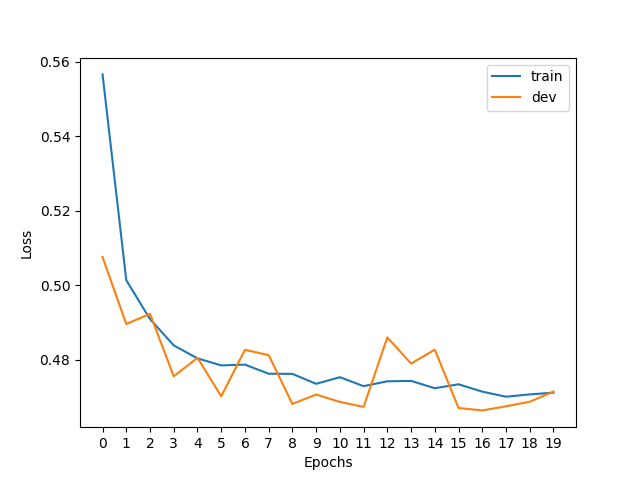
\includegraphics[width=0.45\textwidth]{single_run_loss.png}
   \caption{train and dev loss}
\end{figure}

\noindent\solution{The training loss appears to steadily decrease, which we expect since the model is improving itself with the training data. As for the dev loss, there is a similar beginning drop; however, the curve is much less smooth and fluctuates more with a slight upward trend (and higher loss spikes) toward the later epochs. The difference between the raining loss and dev loss may indicate over-fitting such that the model is becoming too specialized to the training data and thus performs less well with the unseen dev set. Overall, the fluctuations and slight upward trend in the dev loss suggests poor generalization which is may indicate over-fitting or perhaps too high of a learning rate.}

\subsubsection{Run the pipeline: Explore Different Word Embeddings}
As discussed earlier, we initialize the embedding layer of the classifier with pre-trained word embeddings. We have provided in \texttt{main.py} 4 different types of pre-trained word embeddings as different representational options for you to explore their effects on model performance. Again, we provide a visualization function \texttt{visualize\_configs} to depict the performance (dev loss and dev accurracy) across model configurations with different embedding choices. \\\\

\noindent \todo{}: run the \texttt{explore\_embeddings} function in \texttt{main.py}, paste the two plots here, and describe in 2-3 sentences your findings.\\
\noindent \textbf{Hint}: Do you observe any performance differences across different embeddings? What might be the reason of such differences? 
\\\\
\noindent {\color{red}{your plot and answer:}}\\
\begin{figure}[h] 
   \centering
   \subfloat[dev loss]{
       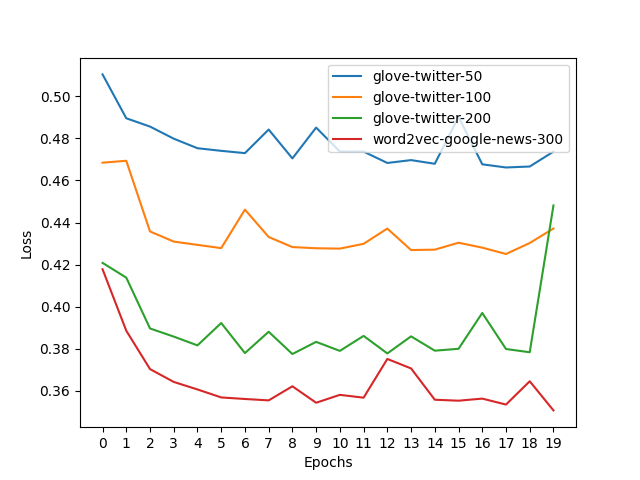
\includegraphics[width=0.45\textwidth]{embedding_loss.png}
       }
   \hfill
   \subfloat[dev accuracy]{
       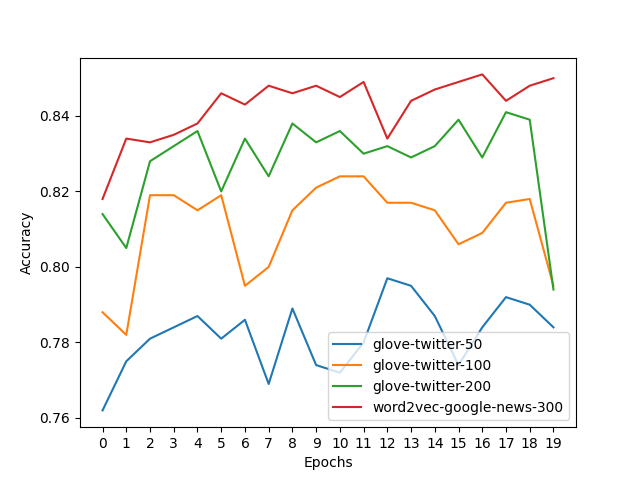
\includegraphics[width=0.45\textwidth]{embedding_acc.png}
       \label{fig:b}
       }
   \caption{loss and accuracy of different pre-trained embeddings}
\end{figure} \\

\noindent\solution{The general downward trend in loss across all embeddings indicates that the models are learning and improving over time. However, the occasional upward spikes suggest fluctuations in the learning process, possibly due to over-fitting, learning rate issues, or the complexity of the data. The bottom embedding (marked red) showed an ending downward trend in dev loss, which might suggest that the model was learning at a slower rate, or the optimizer faced challenges adjusting the weights in the final epochs. The upward trend with occasional downward spikes suggests that the models are gradually improving in terms of prediction accuracy, but there are instances of instability or over-fitting, where the model might memorize data instead of generalizing. The embeddings with a significant decrease in accuracy towards the end of training (marked red) could indicate that the model started to overfit the training data, that there were issues with the learning rate, or the embeddings themselves weren't optimal for the task. All models vary quite largely in their starting and ending losses and accuracy but all maintain a similar downward/upward shape with little to no intersections. The identified performance issues may be a result of the quality of the embeddings (better capture relationships), embedding sizes (pros and cons to different sizes), dataset pre-training relative to target, and varying optimizer behaviors.}

\newpage
\bibliographystyle{apalike}
\bibliography{ref}

\end{document}